\documentclass[tikz, border=10pt]{standalone}
\usepackage{amsmath, amssymb, physics}
\usetikzlibrary{arrows.meta, positioning, shapes.geometric}

\begin{document}

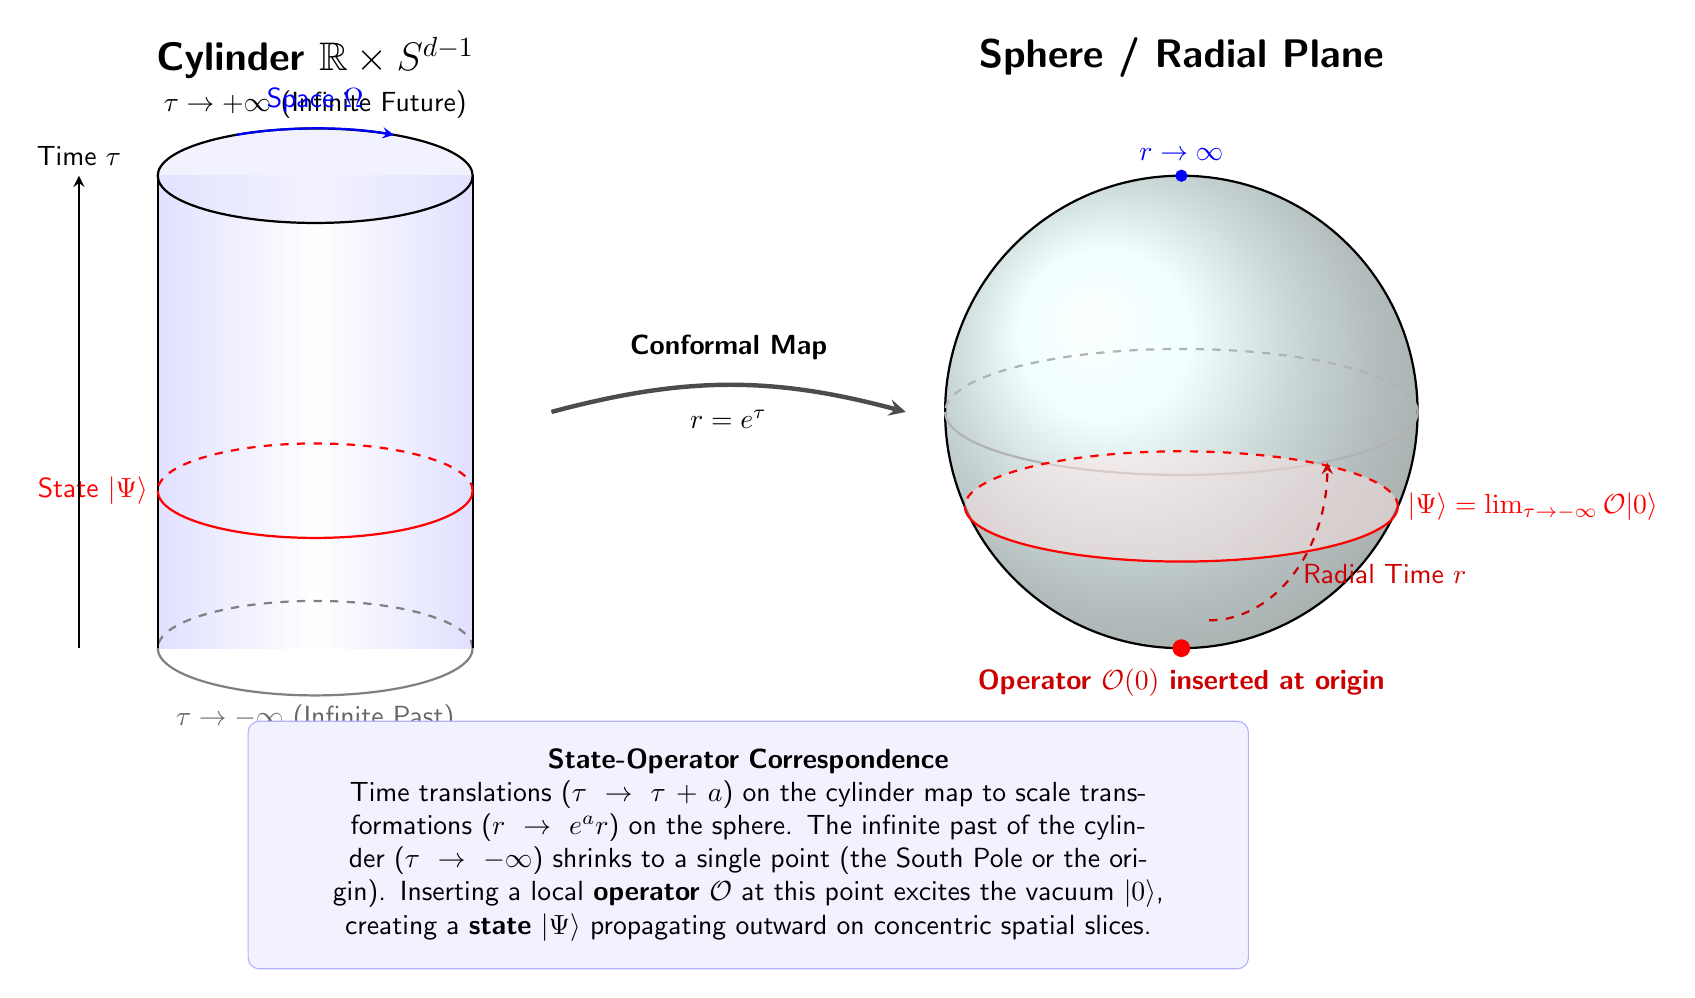
\begin{tikzpicture}[>=stealth, font=\sffamily]

    % -------------------------------------------------------------
    % LEFT SIDE: THE CYLINDER (Spacetime R x S^{d-1})
    % -------------------------------------------------------------
    
    % Shaded background for cylinder
    \shade[left color=blue!20, right color=blue!20, middle color=white, opacity=0.6] 
        (-6, -3) rectangle (-2, 3);
        
    % Bottom Ellipse (Infinite Past)
    \draw[thick, dashed, gray] (-2, -3) arc [start angle=0, end angle=180, x radius=2, y radius=0.6];
    \draw[thick, gray] (-6, -3) arc [start angle=180, end angle=360, x radius=2, y radius=0.6];
    \node[below, text=gray!80!black] at (-4, -3.6) {$\tau \to -\infty$ (Infinite Past)};

    % Top Ellipse (Infinite Future)
    \fill[blue!10, opacity=0.5] (-4, 3) ellipse [x radius=2, y radius=0.6];
    \draw[thick] (-4, 3) ellipse [x radius=2, y radius=0.6];
    \node[above] at (-4, 3.6) {$\tau \to +\infty$ (Infinite Future)};
    
    % Cylinder sides
    \draw[thick] (-6, -3) -- (-6, 3);
    \draw[thick] (-2, -3) -- (-2, 3);

    % Constant Time Slice (The State)
    \draw[thick, dashed, red] (-2, -1) arc [start angle=0, end angle=180, x radius=2, y radius=0.6];
    \draw[thick, red] (-6, -1) arc [start angle=180, end angle=360, x radius=2, y radius=0.6];
    
    % Labels for Cylinder
    \node[red, left] at (-6, -1) {State $|\Psi\rangle$};
    \node[black] at (-4, 4.5) {\Large \textbf{Cylinder $\mathbb{R} \times S^{d-1}$}};
    
    % Time and Space coordinates
    \draw[->, thick] (-7, -3) -- (-7, 3) node[above] {Time $\tau$};
    \draw[->, thick, blue] (-4, 3) ++(120:2 and 0.6) arc [start angle=120, end angle=60, x radius=2, y radius=0.6] node[midway, above=2pt] {Space $\Omega$};

    % -------------------------------------------------------------
    % MIDDLE: CONFORMAL MAP ARROW
    % -------------------------------------------------------------
    
    \draw[->, ultra thick, draw=black!70] (-1, 0) to[bend left=15] 
        node[midway, above=5pt] {\textbf{Conformal Map}}
        node[midway, below=5pt] {$r = e^\tau$} (3.5, 0);

    % -------------------------------------------------------------
    % RIGHT SIDE: THE SPHERE (Mapped Spacetime / Radial Quantization)
    % -------------------------------------------------------------
    
    \def\sphereradius{3}
    \def\spherecenterX{7}
    \def\spherecenterY{0}
    
    % Sphere Title
    \node[black] at (\spherecenterX, 4.5) {\Large \textbf{Sphere / Radial Plane}};
    
    % 3D Sphere Shading
    \shade[ball color=cyan!15, opacity=0.5] (\spherecenterX, \spherecenterY) circle (\sphereradius);
    
    % Sphere Outline
    \draw[thick] (\spherecenterX, \spherecenterY) circle (\sphereradius);
    
    % Equator (for 3D perspective)
    \draw[thick, dashed, gray!60] (\spherecenterX+\sphereradius, \spherecenterY) arc [start angle=0, end angle=180, x radius=\sphereradius, y radius=0.8];
    \draw[thick, gray!60] (\spherecenterX-\sphereradius, \spherecenterY) arc [start angle=180, end angle=360, x radius=\sphereradius, y radius=0.8];
    
    % Mapped Time Slice (The State as a Latitude Line)
    % Calculate radius of the slice at y = -1.2 to match tau = -1
    \def\sliceY{-1.2}
    \def\sliceR{2.749}
    
    % Mapped State Slice (Using robust key-value syntax)
    \fill[red!10, opacity=0.5] (\spherecenterX, \sliceY) ellipse [x radius=\sliceR, y radius=0.7];
    \draw[thick, dashed, red] (\spherecenterX+\sliceR, \sliceY) arc [start angle=0, end angle=180, x radius=\sliceR, y radius=0.7];
    \draw[thick, red] (\spherecenterX-\sliceR, \sliceY) arc [start angle=180, end angle=360, x radius=\sliceR, y radius=0.7];
    
    % Labels for the Sphere
    \node[red, right] at (\spherecenterX+\sliceR, \sliceY) {$|\Psi\rangle = \lim_{\tau \to -\infty} \mathcal{O}|0\rangle$};
    
    % Operator Insertion (South Pole)
    \filldraw[red] (\spherecenterX, -\sphereradius) circle (3pt);
    \node[below=4pt, text=red!80!black] at (\spherecenterX, -\sphereradius) {\textbf{Operator $\mathcal{O}(0)$ inserted at origin}};
    
    % North Pole
    \filldraw[blue] (\spherecenterX, \sphereradius) circle (2pt);
    \node[above=2pt, text=blue] at (\spherecenterX, \sphereradius) {$r \to \infty$};
    
    % Radial Arrow on the sphere surface
    \draw[->, thick, dashed, red!80!black] (\spherecenterX, -\sphereradius) ++(45:0.5) arc [start angle=-90, end angle=0, x radius=1.5, y radius=2] node[midway, right] {Radial Time $r$};

    % -------------------------------------------------------------
    % EXPLANATORY TEXT BLOCK
    % -------------------------------------------------------------
    \node[align=center, text width=12cm, fill=blue!5, draw=blue!30, rounded corners, inner sep=10pt] 
    at (1.5, -5.5) {
        \textbf{State-Operator Correspondence}\\
        Time translations ($\tau \to \tau + a$) on the cylinder map to scale transformations ($r \to e^a r$) on the sphere. The infinite past of the cylinder ($\tau \to -\infty$) shrinks to a single point (the South Pole or the origin). Inserting a local \textbf{operator} $\mathcal{O}$ at this point excites the vacuum $|0\rangle$, creating a \textbf{state} $|\Psi\rangle$ propagating outward on concentric spatial slices.
    };

\end{tikzpicture}

\end{document}
